% https://www.overleaf.com/learn/latex/Learn_LaTeX_in_30_minutes
\documentclass{article}
\usepackage{graphicx}
\usepackage{hyperref}


\title{My first LaTeX document}
\author{Hubert Farnsworth\thanks{Funded by the Overleaf team.}}
\date{12-12-2022}

\begin{document}
\maketitle
\tableofcontents

\section{Section 1: My First Section}

some text for explaining this section.

\subsection{Text Style}

Normal text

\textbf{Bold text}

\textit{Italic text}

\underline{underline}

Emphasizing

Normal sentence \emph{emph}.

\textit{Italic sentence \emph{emph}.}

\textbf{Bold sentence \emph{emph}.}

\subsection{Figure}

Refer to figure~\ref{fig:brainlab-logo}

\begin{figure}[ht!]
    \centering
    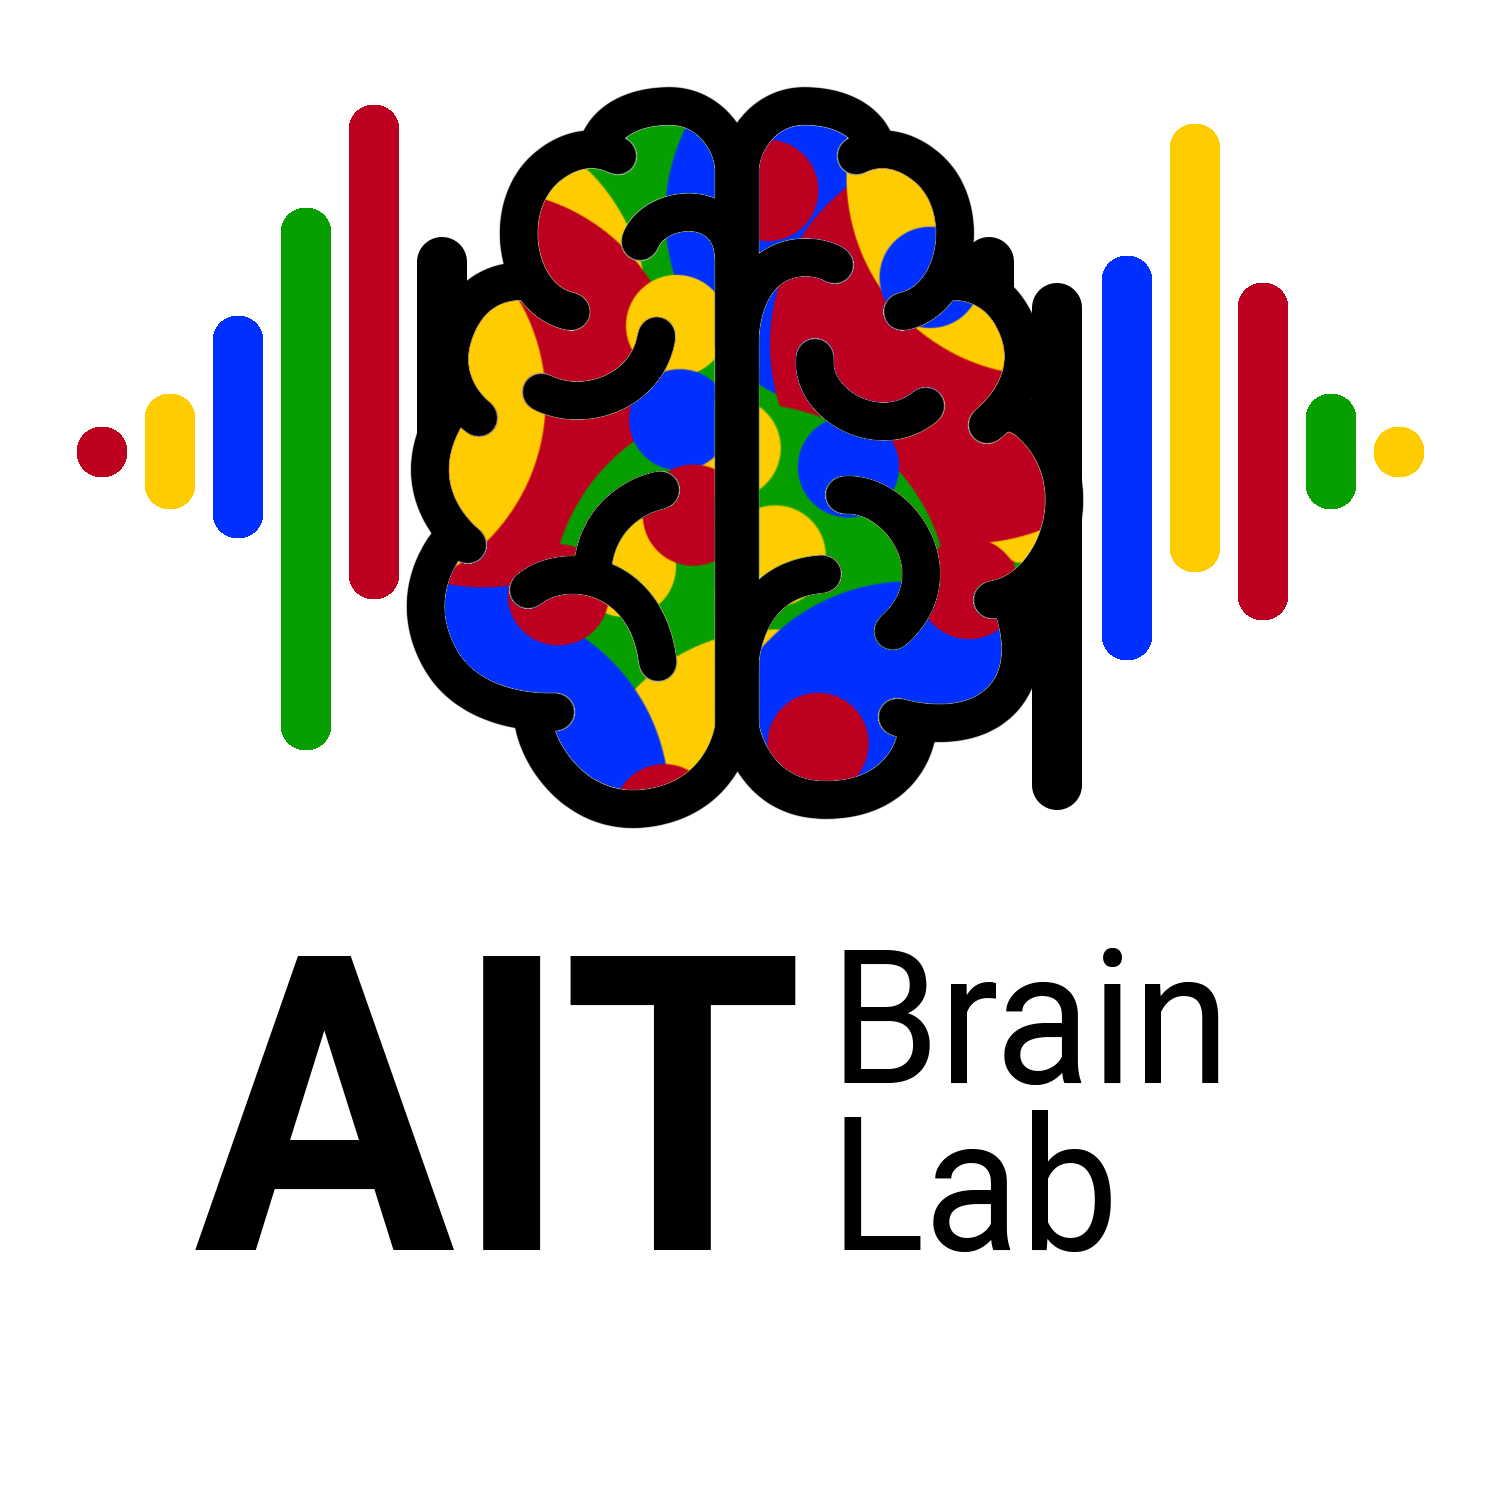
\includegraphics[width=0.75\textwidth]{../4_figure/figures/bci-logo.png}
    \caption{AIT Brainlab Logo}
    \label{fig:brainlab-logo}
\end{figure}


\subsection{Table}

Refer to table~\ref{tab:demo-table}

\begin{table}[ht!]
    \begin{center}
        \begin{tabular}{||c c c c||} 
        \hline
        Col1 & Col2 & Col2 & Col3 \\ [0.5ex] 
        \hline\hline
        1 & 6 & 87837 & 787 \\ 
        \hline
        2 & 7 & 78 & 5415 \\
        \hline
        3 & 545 & 778 & 7507 \\
        \hline
        4 & 545 & 18744 & 7560 \\
        \hline
        5 & 88 & 788 & 6344 \\ [1ex] 
        \hline
        \end{tabular}
    \caption{\label{tab:demo-table}Your caption.}
    \end{center}
\end{table}


\end{document}